% !TeX spellcheck = en_US
% !TeX encoding = UTF-8
\documentclass{beamer}

\mode<presentation> { \usetheme{Madrid} }

\usepackage{graphicx, graphics}
\usepackage{apacite}
\usepackage[style=iso]{datetime2}
\DeclareGraphicsExtensions{.pdf, .png, .jpg, .gif}

\title[Cavity]{Helixco Cavity}

\author{Jaewoong Lee}
\institute[UNIST]
{
	Ulsan National Institute of Science and Technology
	\medskip
	\newline
	\textit{jwlee230@unist.ac.kr}
}
\date{\today}

\begin{document}
    \begin{frame}
        \titlepage
    \end{frame}

	\begin{frame}
        \frametitle{Overview}
        \tableofcontents
    \end{frame}

    \section{Methods}
    \begin{frame}
        \frametitle{t-SNE}

        \begin{figure}[h!]
            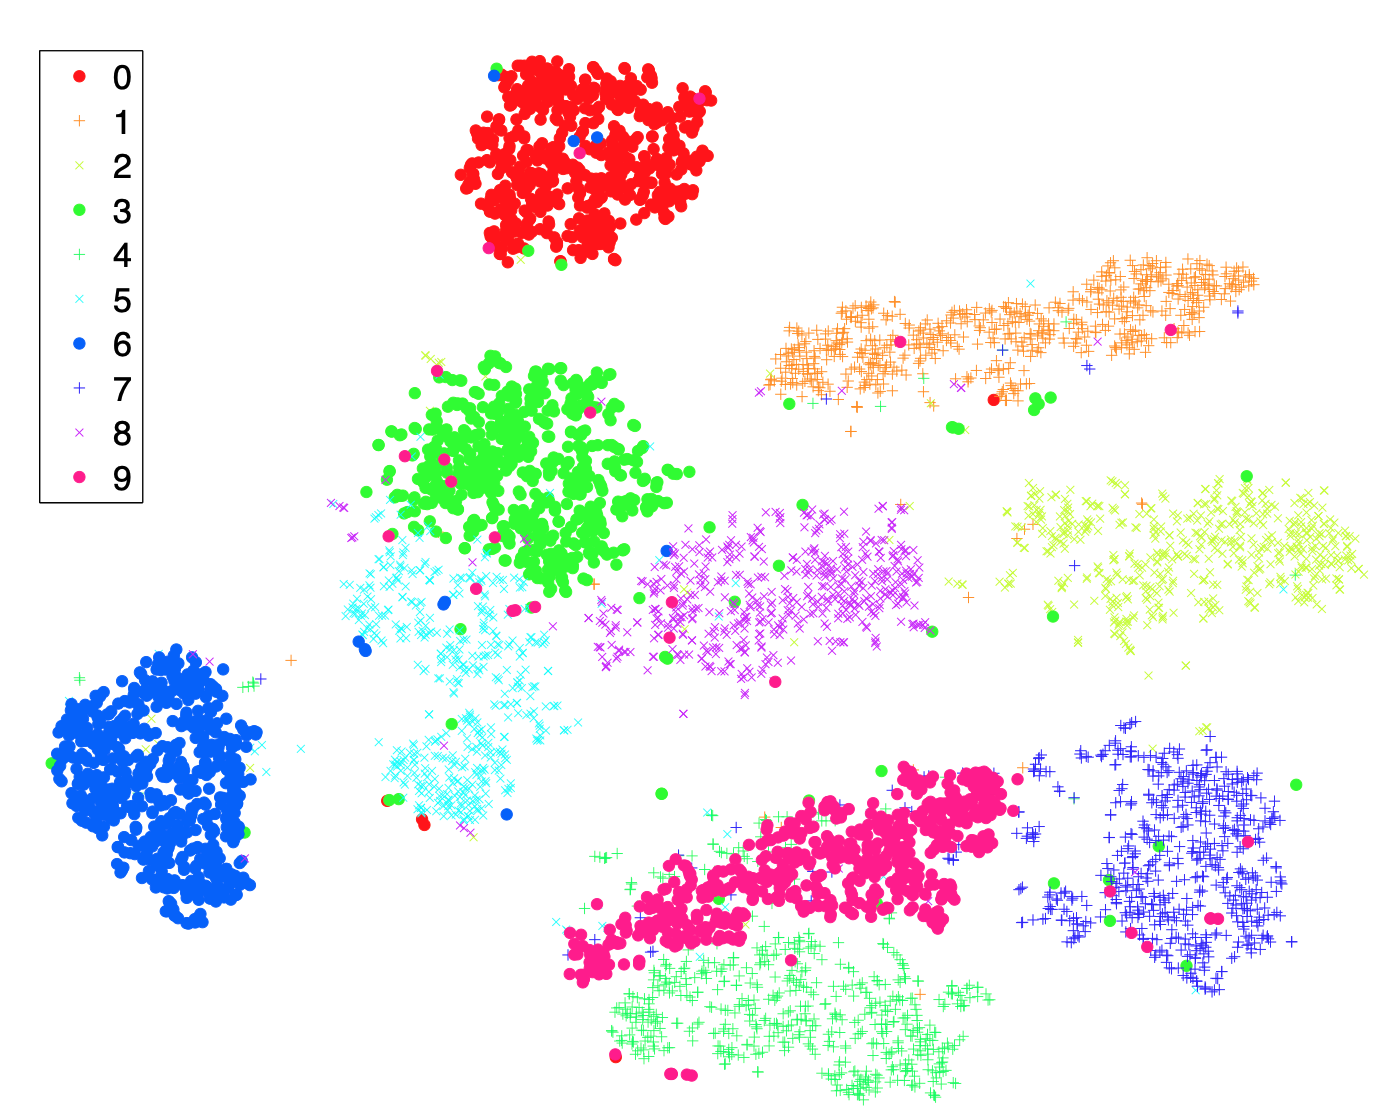
\includegraphics[width=0.6 \linewidth]{figures/mnist.png}
            \caption{Visualizations of handwritten digits from the MNIST data set \protect \cite{tsne1}}
        \end{figure}
    \end{frame}

    \begin{frame}
        \frametitle{Programming Methods}

        \begin{itemize}
            \item Docker \cite{docker1}
            \item QIIME 2
            \item Scikit-learn \cite{sklearn1, sklearn2}
        \end{itemize}
    \end{frame}

    \begin{frame}
        \frametitle{QIIME 2 Workflow}

        \begin{figure}[h!]
            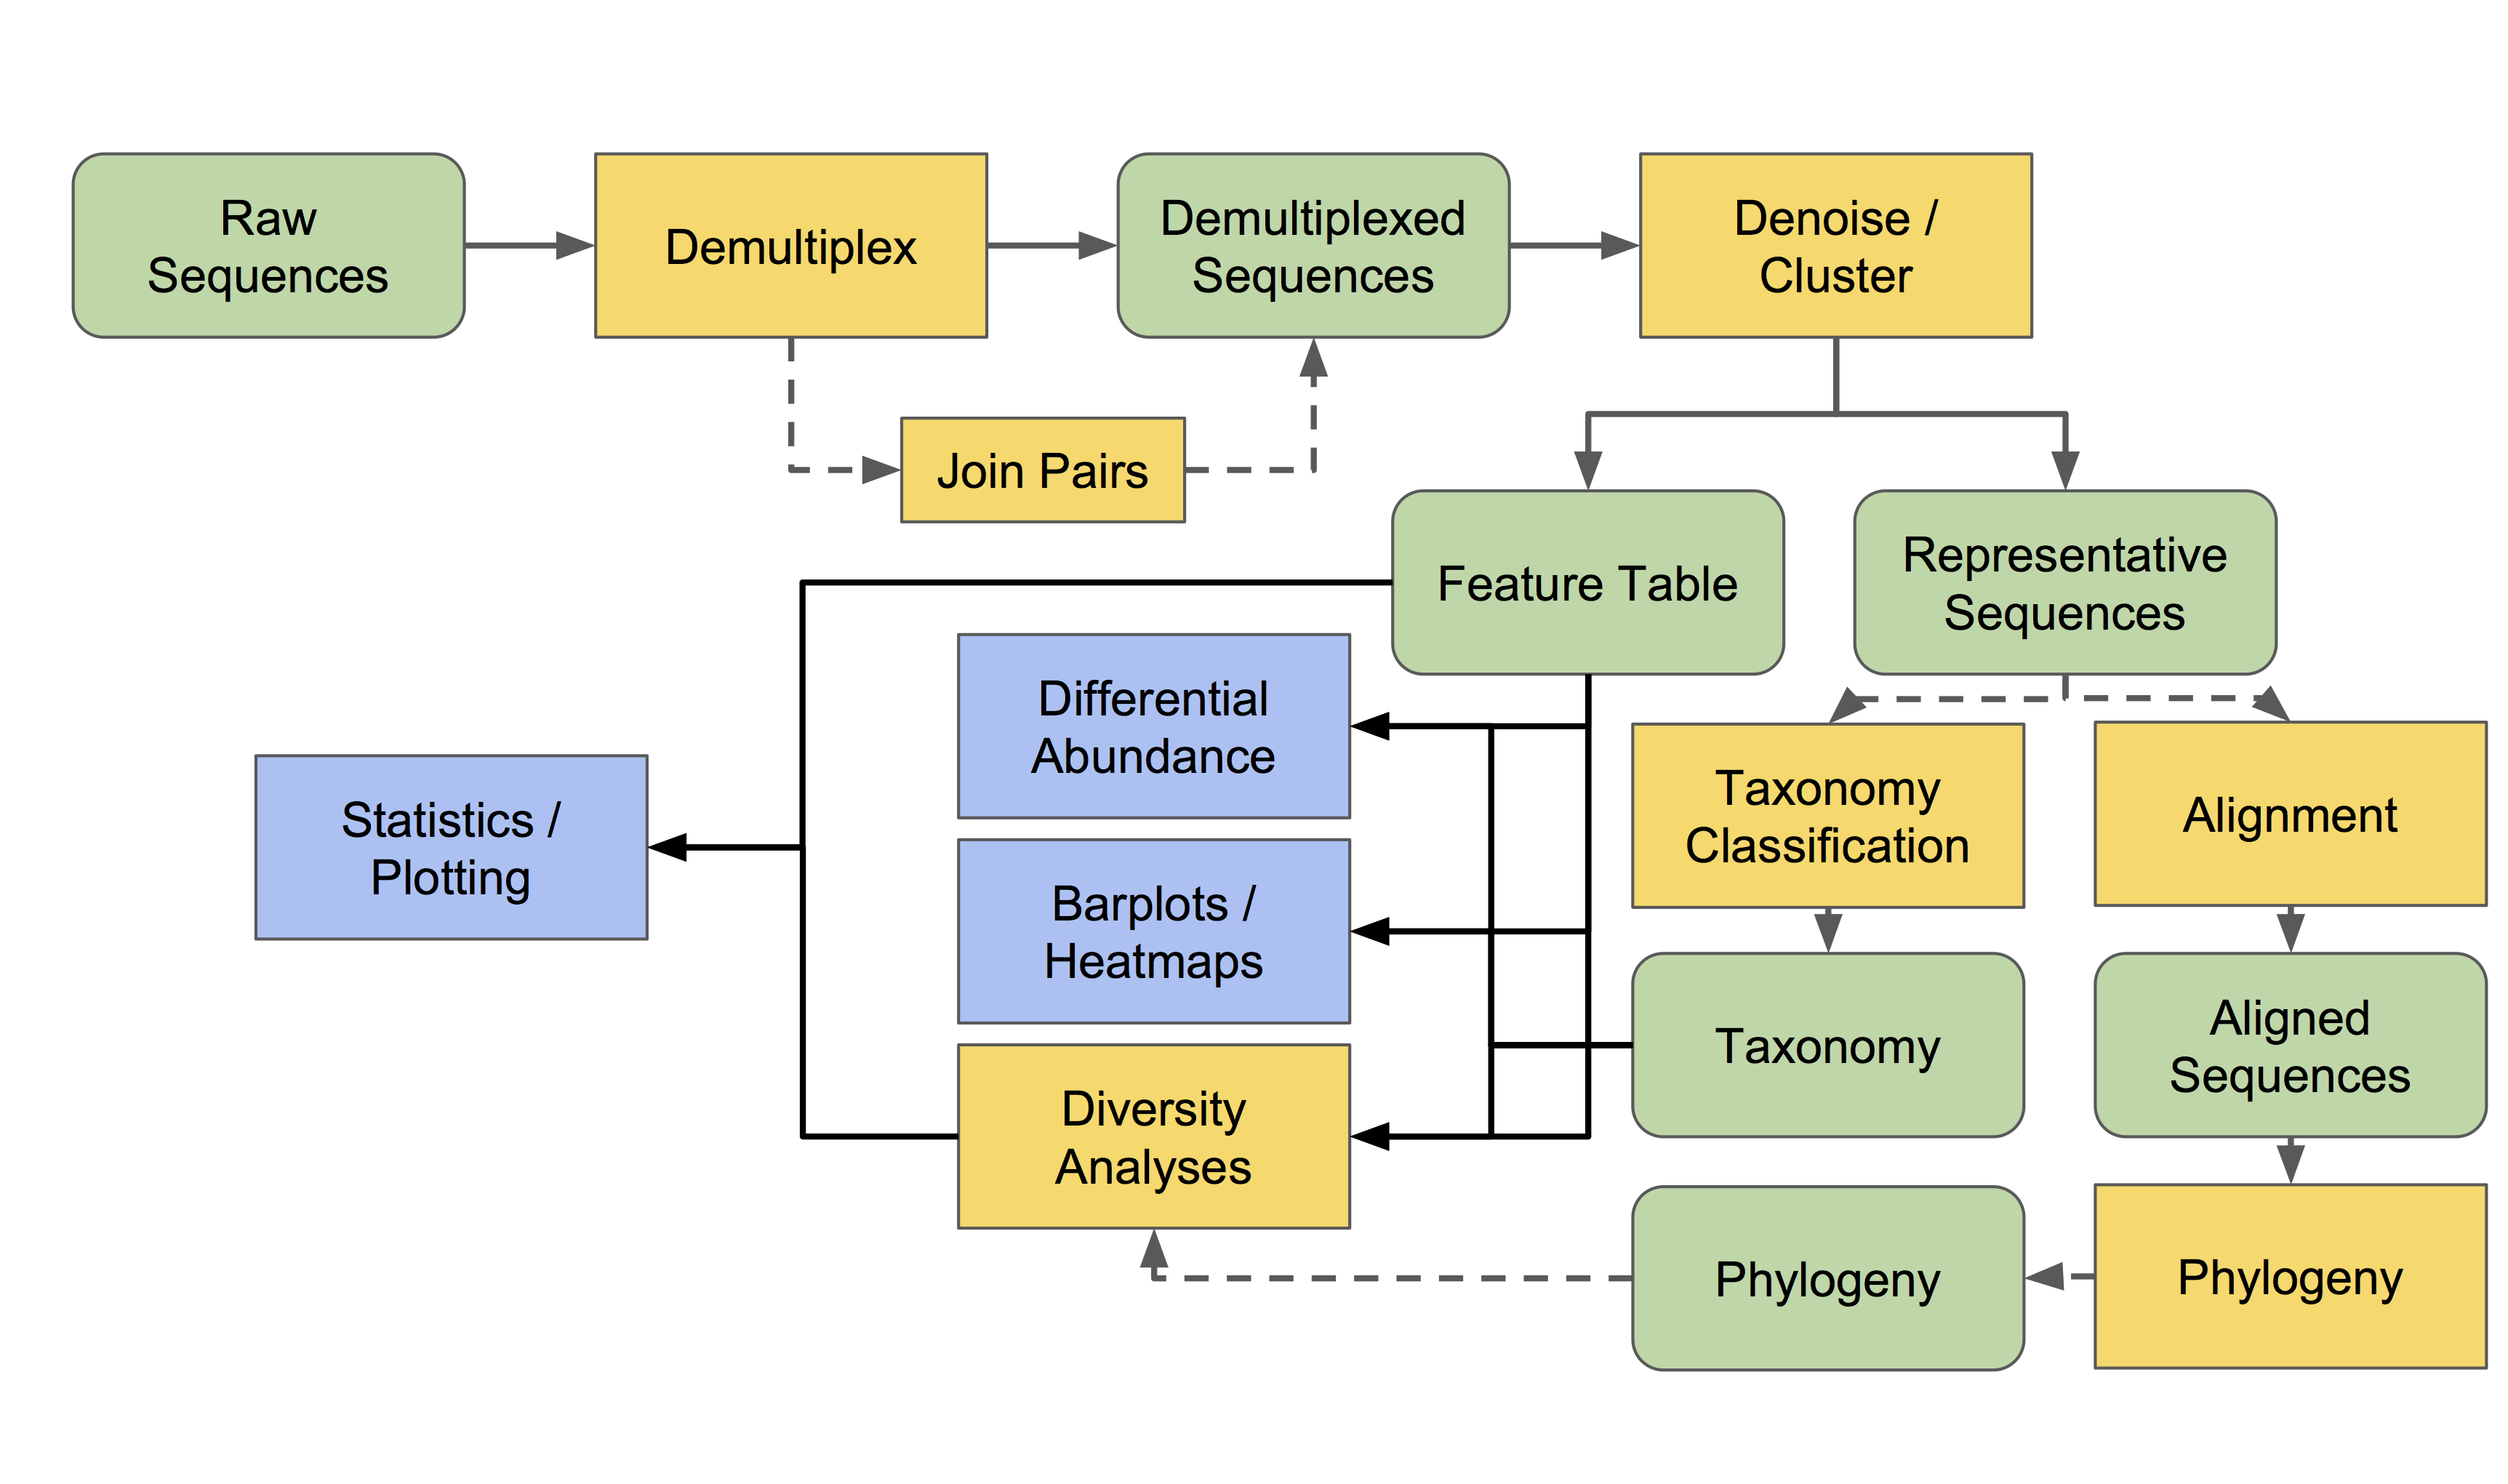
\includegraphics[width=0.8 \linewidth]{figures/workflow.png}
            \caption{QIIME 2 Workflow}
        \end{figure}
    \end{frame}

    \section{Proceedings}
    \begin{frame}[allowframebreaks]
        \frametitle{Yields}

        \begin{itemize}
            \item t-SNE with every bacterium
        \end{itemize}
    \end{frame}

    \begin{frame}
        \frametitle{t-SNE with every bacterium}

        \begin{figure}
            $\begin{array}{cc}
                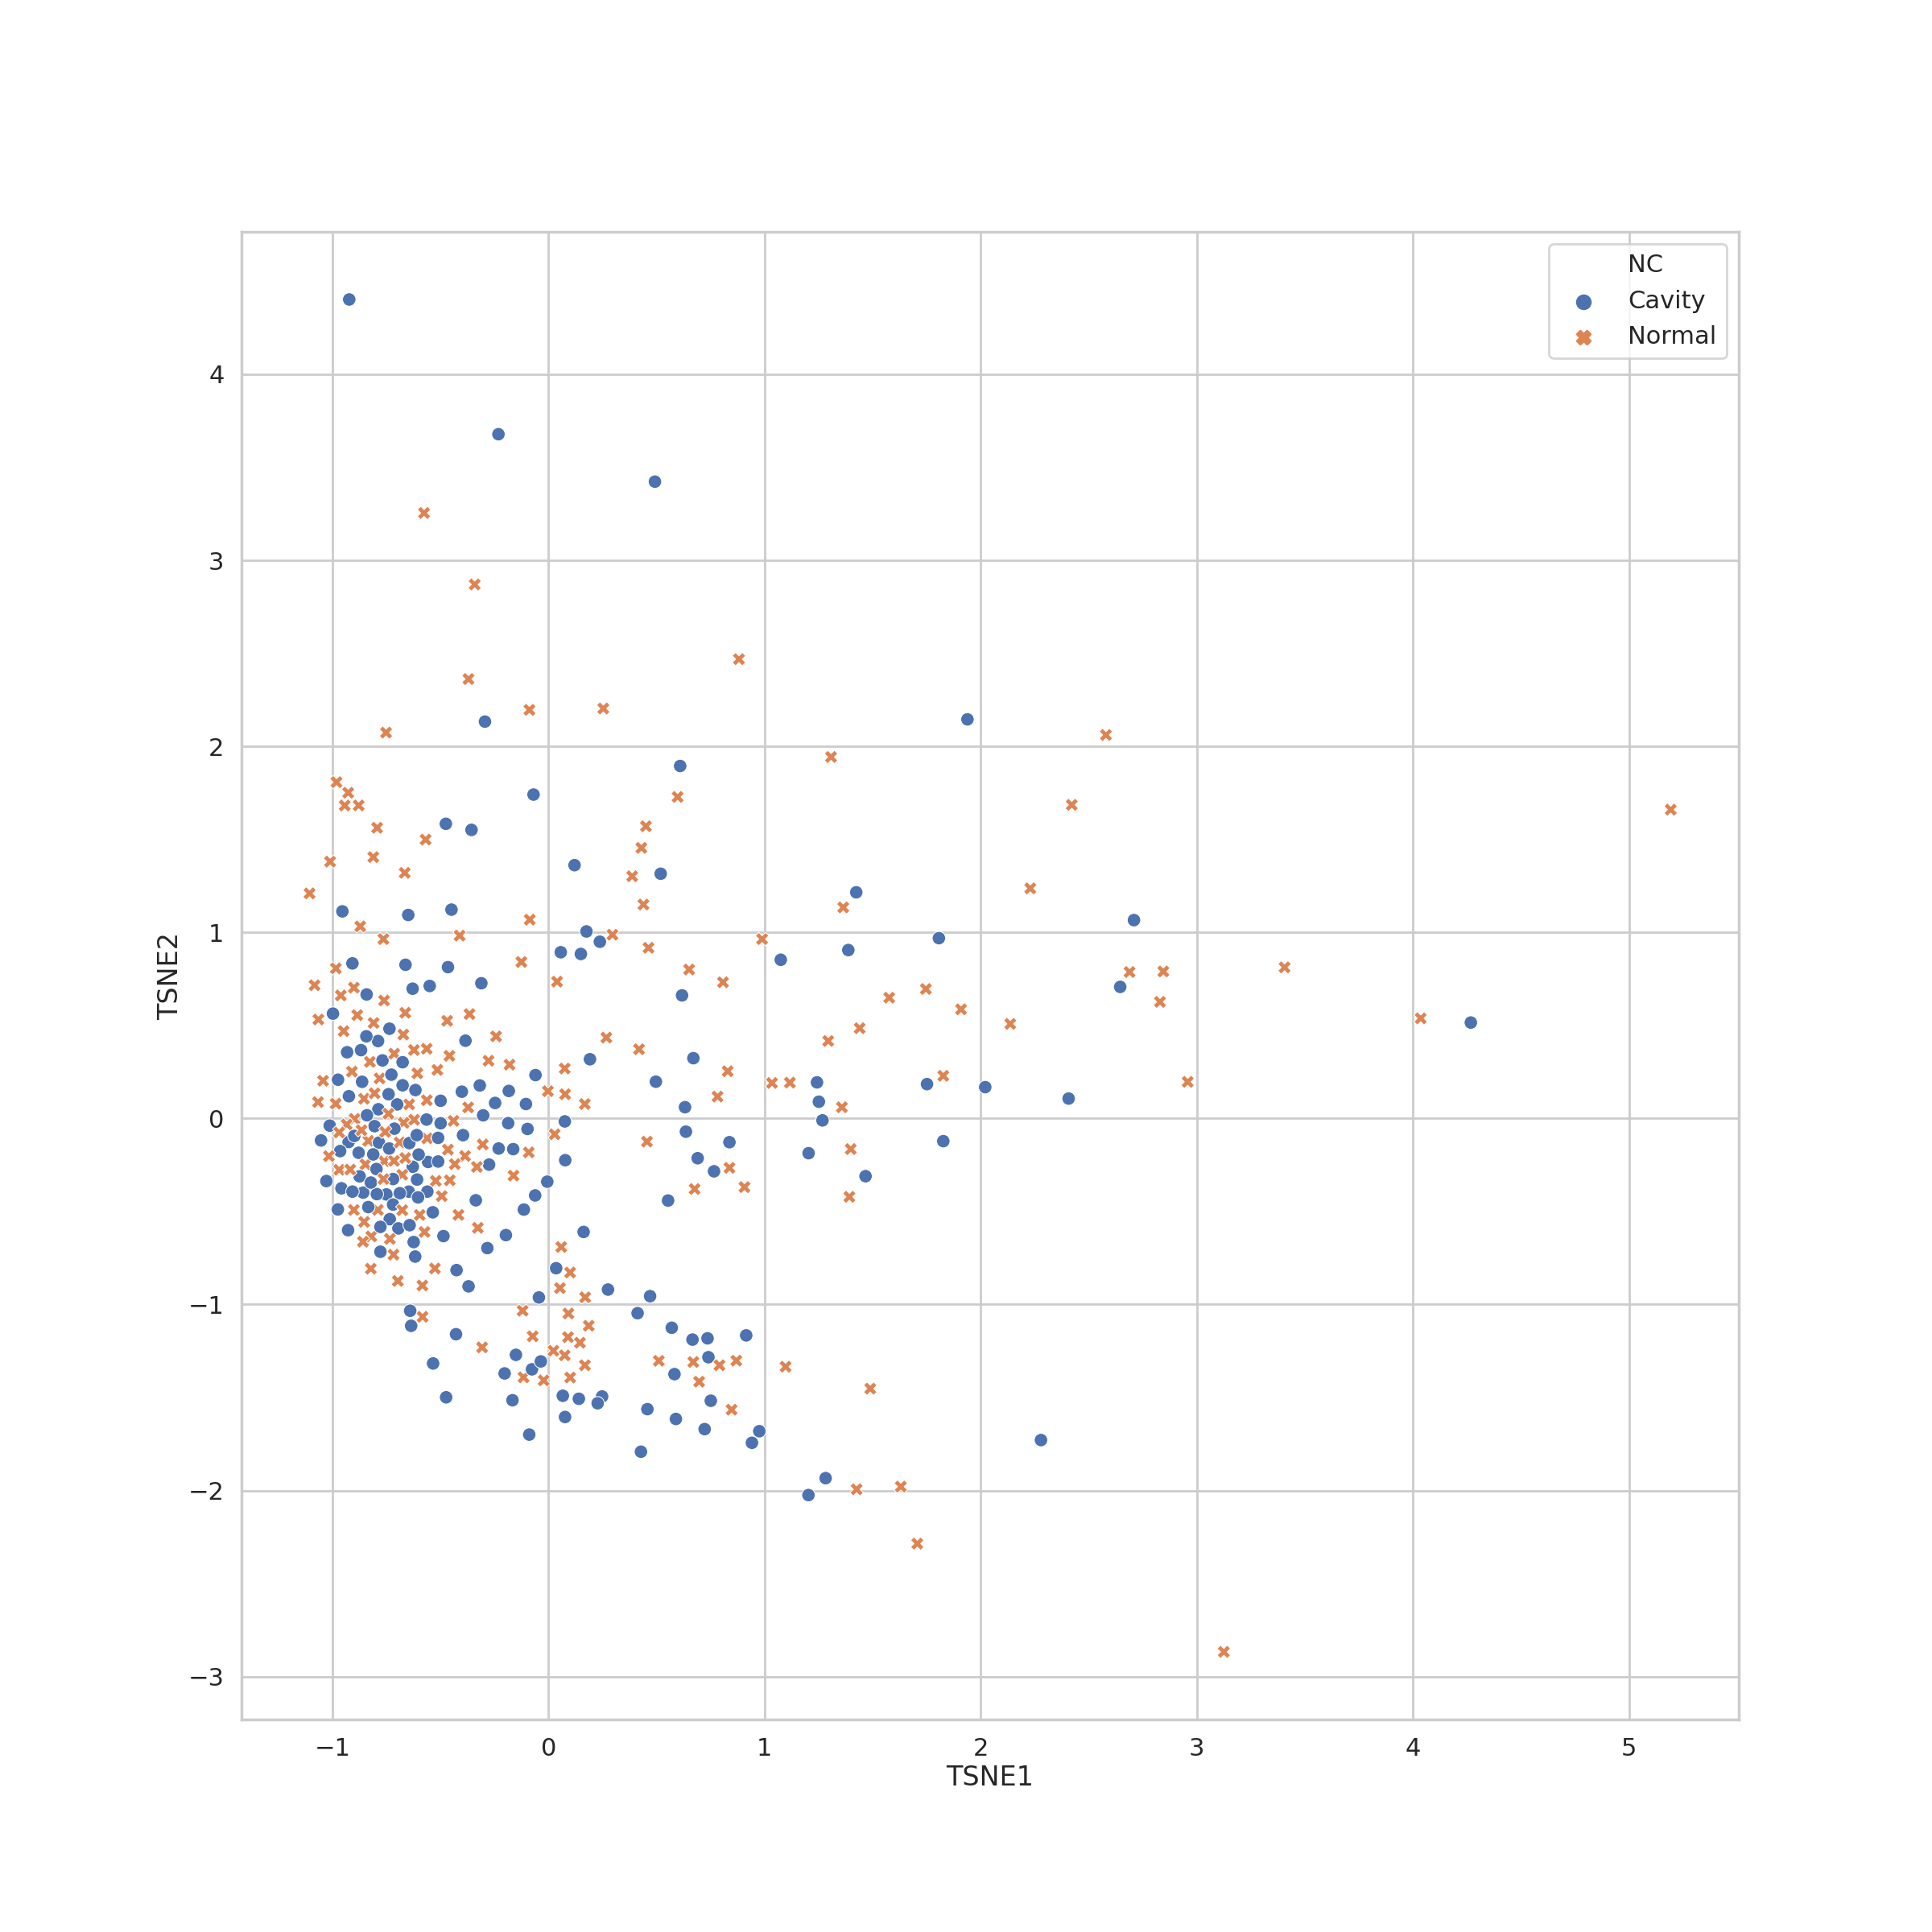
\includegraphics[width=0.4 \linewidth]{figures/step14/NC.png}
                &
                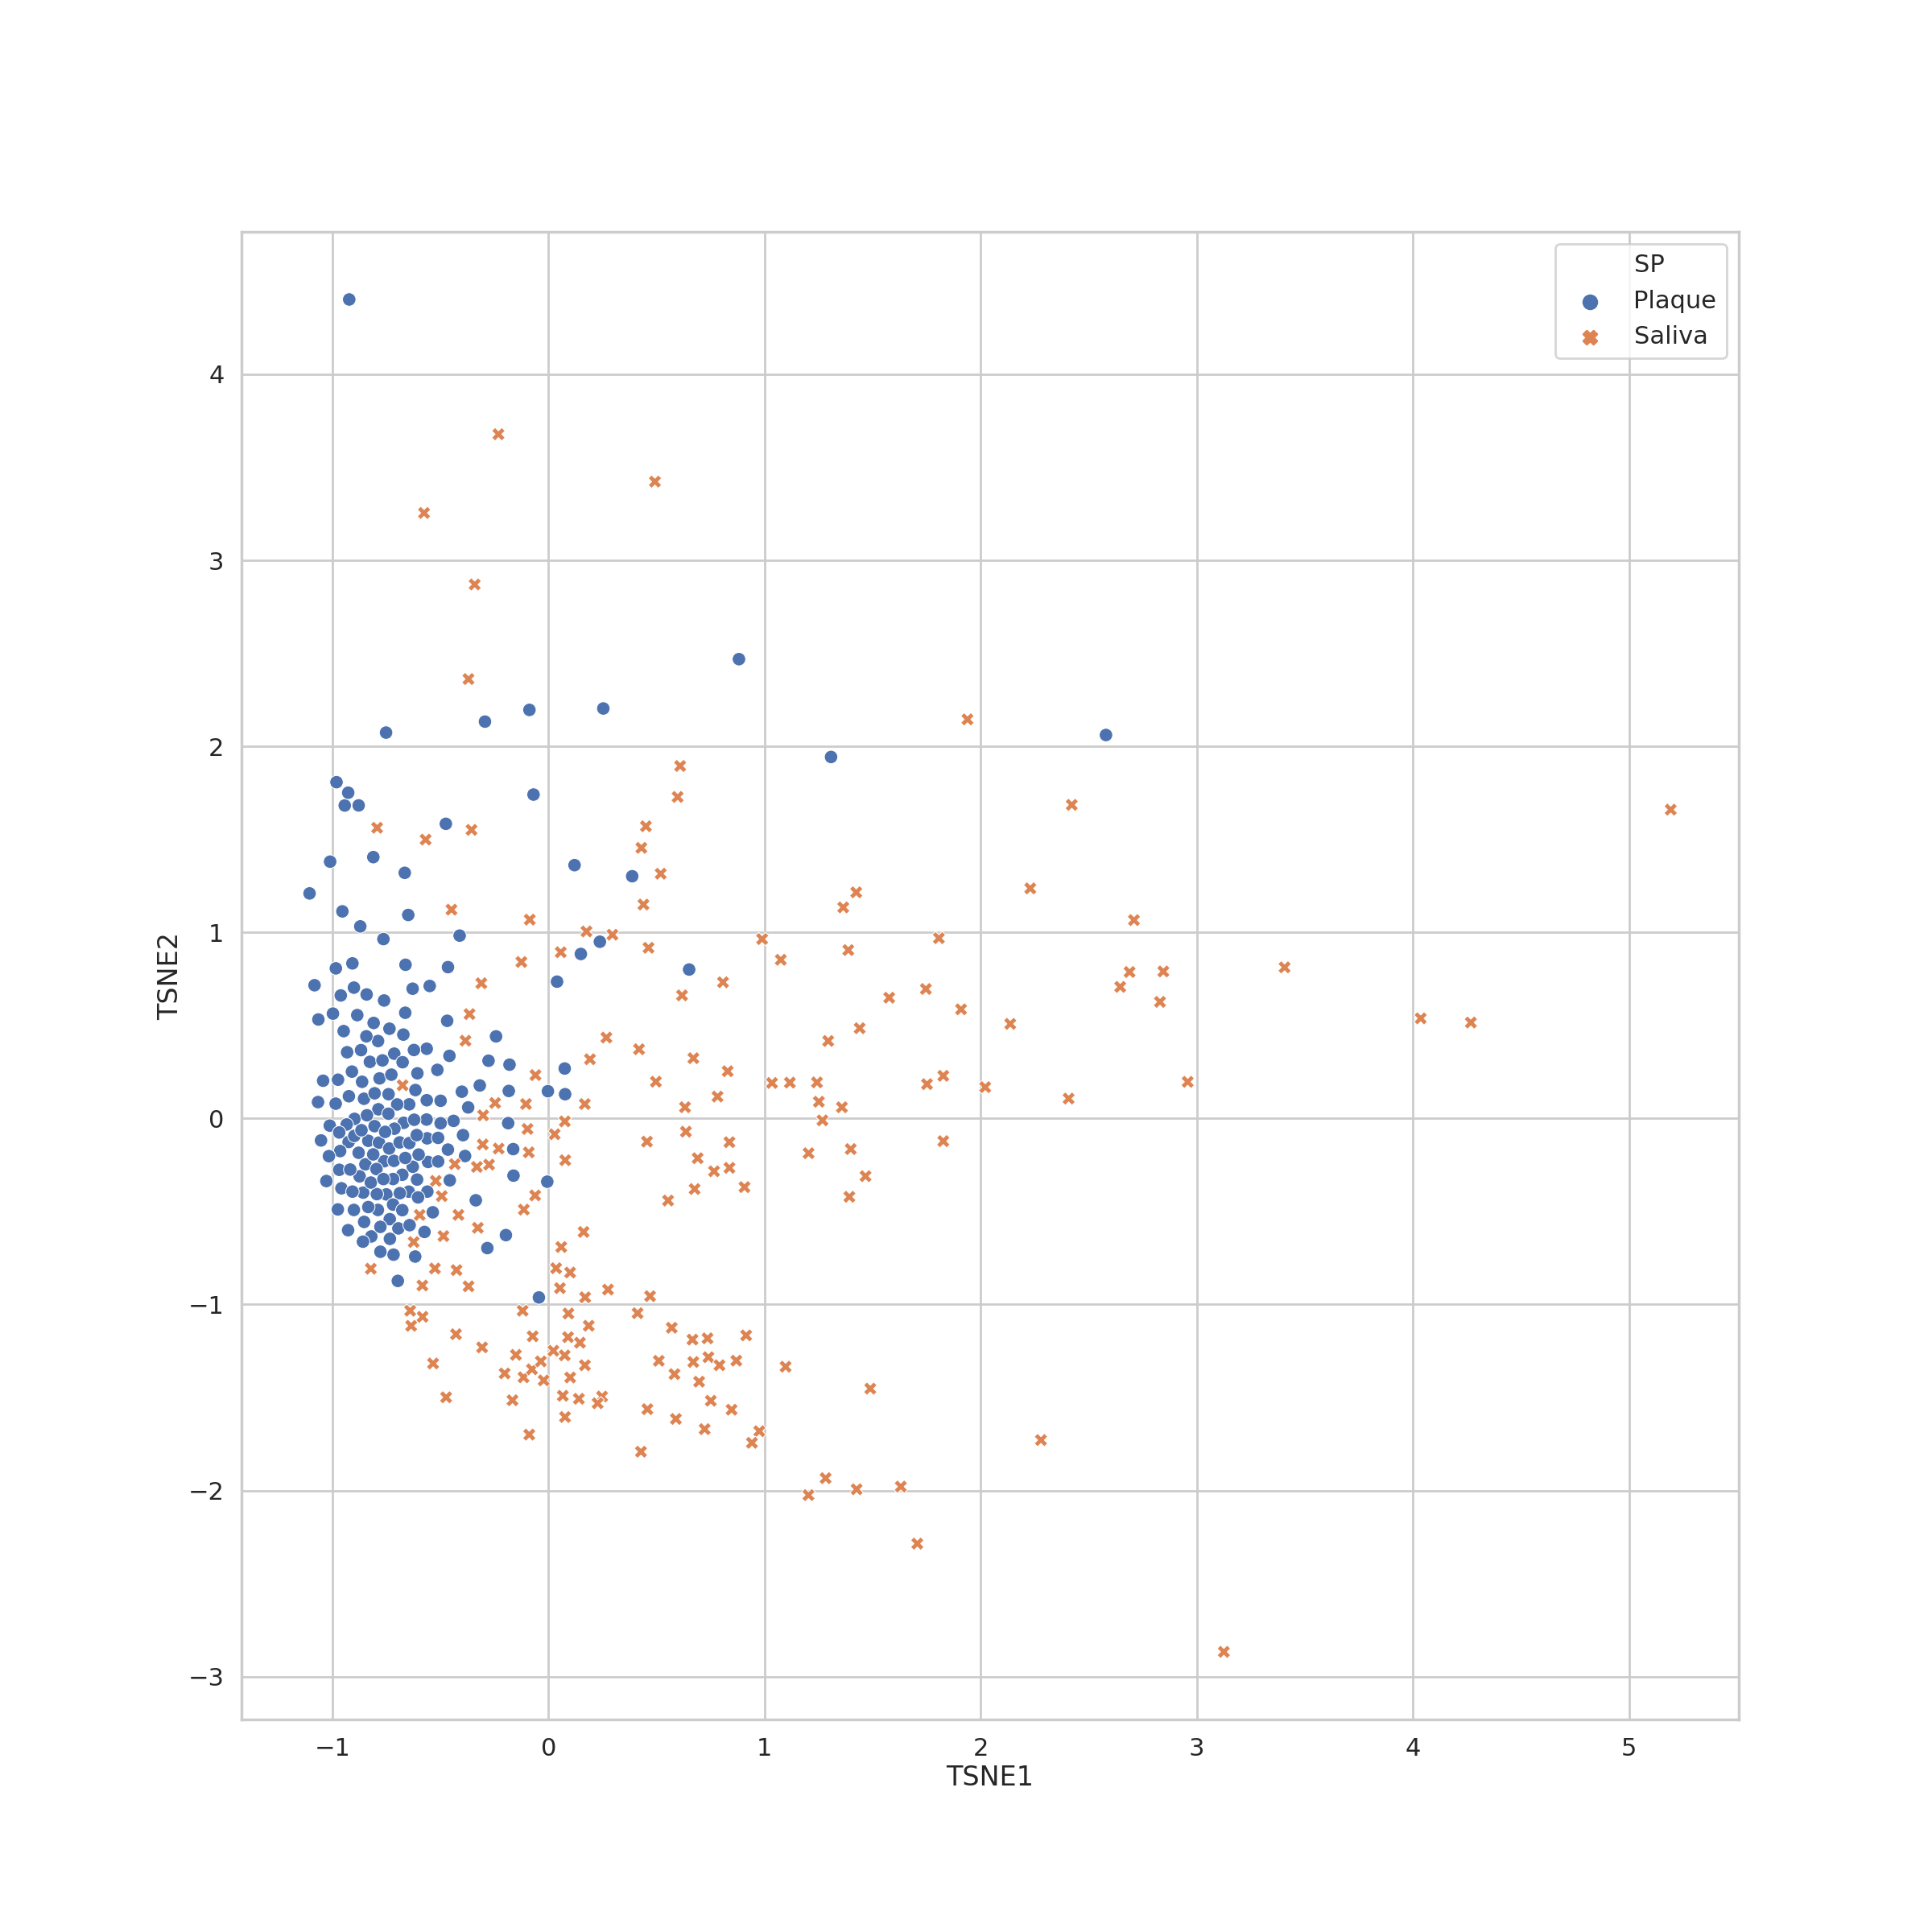
\includegraphics[width=0.4 \linewidth]{figures/step14/SP.png}
                \\
                \mbox{(a) Normal vs. Cavity} & \mbox{(b) Saliva vs. Plaque}
            \end{array}$
        \end{figure}

        $\therefore$ We need to select bacteria with feature importance.
    \end{frame}

    \begin{frame}[allowframebreaks]
        \frametitle{Requirements}

        \begin{figure}[h!]
            
\includegraphics[width=0.5 \linewidth]{figures/time.png}
        \end{figure}
    \end{frame}

    \begin{frame}[allowframebreaks]
        \frametitle{Expectations}

        \begin{itemize}
            \item Improved classification
        \end{itemize}
    \end{frame}

   	\begin{frame}[allowframebreaks]
        \frametitle{References}
        \bibliographystyle{apacite}
        \bibliography{reference}
    \end{frame}
\end{document}